\iffalse
\bibliography{reference/refs}
\fi


\chapter{Related Works}
\label{chap:relatedWorks}
	Numbers of research works related to face de-identification have been 
	published. For images and videos, the challenges are different. 
	In this chapter, the previous face algorithms for images and videos 
	are described individually in section \ref{sec:APPimages} and section
	\ref{sec:APPvideos}. 

\section{Approaches for Images}
\label{sec:APPimages}
	For images, the most important point is to keep balance between privacy
	protection and data utility preservation. For example, a face image 
	shows a person is smiling in frontal pose. After de-identifcation, the 
	person should not be recognized as the original one, but still smile in
	frontal pose.

	The existing algorithms for face de-identification in images falls into
	three categories: ad-hoc approaches, $k$-same framework and  other face 
	synthesis approaches. 

	\subsection{Ad-hoc Approaches}
	
	As the most intuitive idea of hiding information, image distortion is widely
	used to protect privacy. By destorying the original image information, image
	distortion algorithms make a trade off between privacy information and image 
	quality. General face recognition algorithms find out the identity by 
	computing the similarity between a target image and the images in database. 
	The ad-hoc approaches could protect privacy since the original information 
	has been altered. In traditional broadcast media, such as TV interview and 
	newspapers, the privacy related region is obfuscated to prevent the leak risking 
	of privacy information. This section introduces the ad-hoc approaches including 
	pixelation, blurring, scrambling, masking, cartoon, and encryption. 

	{\it Pixelation and blurring}. The pixelation method subsamples the image by 
	replacing all pixels within a 
	block region with one pixel. In other words, one image is covered by multiple
	patches \cite{Boyle00}. In early computer graphic applications, such as graphic
	games, the pictures appear at very low resolutions, looking like pixelation.
	Blurring method smoothes images with some filters like Gaussian filter or 
	average filter ~\cite{Agrawal09,blur05}. This method alters a pixel value 
	according to its neighbour pixels. As a consequence, the processed image is
	visually fuzzy. To be more specific, the Gaussian filter is:
	\begin{equation}
    \label{equ:gaussian}
      \begin{aligned}
      		G(x,y) = \frac{1}{2\pi\sigma^2} e^{-\frac{(x^2+y^2)}{2\sigma^2}},
      \end{aligned}
    \end{equation}
    where $\sigma$ is the standard deviation, $x,y$ are the distances from the 
    origin in the horizontal and vertical axis separately. This equation would
    produce a weight matrix which would be used to filter the whole image.

	Although these two methods are widely used in practical situations like TV 
	interviews and newspapers, they suffer from the same risk proposed in ~\cite{Newton05} 
	called {\it parrot attack}. Blurring and pixelation destory a target image 
	information so that the target image is not similar to any image in database. 
	Parrot attack would preprocess all the database images with the same pixelation or 
	blurring, then applies face recognition algorithms to pixelated or blurred 
	images. Because the target image and the images in database are both processed
	with similar procedures, the recognition ratio increases sharply. 

	{\it Scrambling}. Dufaux ~\cite{dufaux08} introduced a privacy protection method 
	by scrambling 
	the locations of pixels or Fourier coefficients within a rectangle range. By 
	controling the range size, different degrees of fuzzy results could be produced. 
	It is possible to recover the original image information if the scrambling order 
	is recorded. Essentially, the scrambling method is a kind of encryption with 
	the permutation order as the encryption key. Scrambling method overcomes other 
	traditional encryption methods in original information preserving. If the 
	scrambling range is in proper size, although the result is still unnatural, 
	the original information is understandable.
	In other words, scrambling also trades privacy protection with data utility. 
	The images shown in Figure \ref{fig:adhoc_example} retriving from \cite{dufaux10} 
	illustrate the examples of different de-identification methods introduced in
	the above content. 

	\begin{figure}[!htb]
	    \centering
	    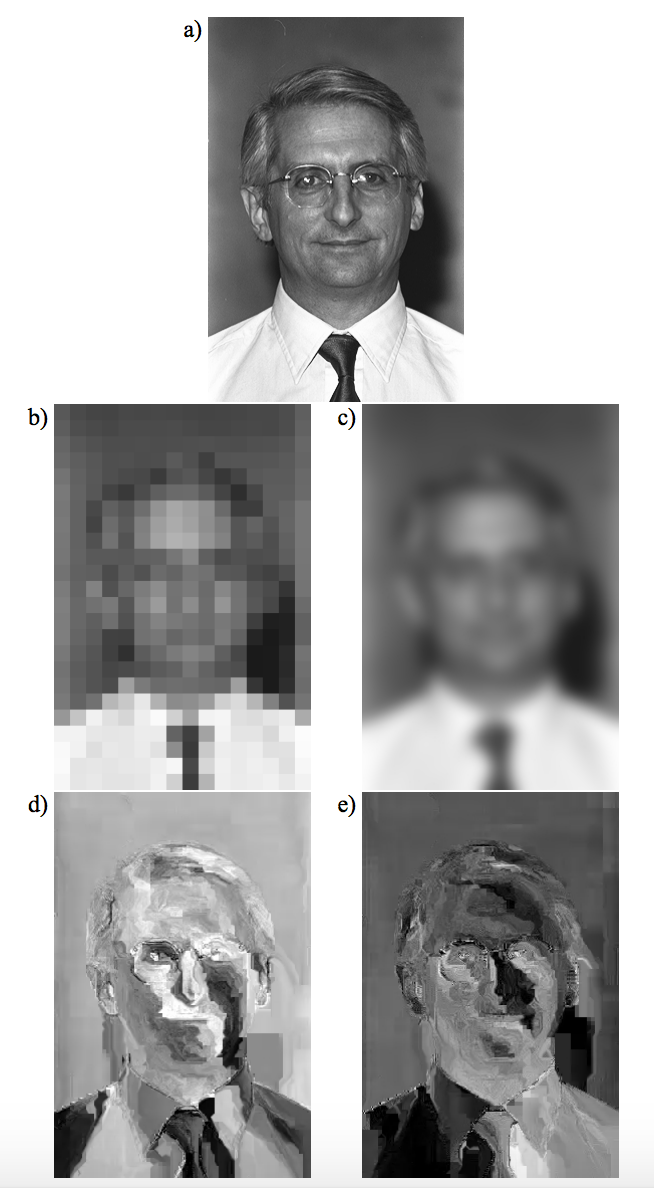
\includegraphics[scale=0.8]{figure/adhocVertical}
	    \caption{Ad-hoc Approaches \cite{dufaux10}. (a) Original image. (b) Pixelation.
	    (c) Blurring. (d) Scrambling in pixels. (e) Scrambling in Fourier coefficients.}
	    \label{fig:adhoc_example}
  	\end{figure}

	{\it Masking}. A traditional approach of protection privacy is to cover
	the region of interest (hereinafter referred to as ROI) with a mask. The
	mask types are various, many examples are listed in \cite{Winkler14}. The
	intuitive masking method in face de-identificaiton is to cut the face 
	region off and replace the region with black color. It also could be 
	extended to paint the ROI, like face, with background images  
	\cite{inpaint09,Qureshi09}. After the processing, the ROI is totally
	ereased as nothing existed. 

	{\it Cartooning.} Converting a real image into cartooning one is 
	a developed technology. Erdélyi ~\cite{erdely14} applied this 
	technology in de-identification area by applying edge detector 
	and mean-shift algorithm in the real image so that the pixels 
	with similar colors would be assign the same value. It is intuitive 
	that cartooning method is able to thwart automatic face recognition 
	algorithms. However, it is hardly deceive a human. 

	{\it Encryption}. Compared with other de-identification methods 
	introduced before, encryption has the advantage in recovery ability 
	\cite{Boult05}. The ROI in image is encrypted to produce snowboard. 
	With a proper key, the encrypted image is always available to be 
	decrypted so that the image remains useful when required. The 
	shortcoming is extra space would be taken to store the encryption
	key. Furthermore, the processed data is still not visual natural. 

	As a summation, the previous de-identification methods are all trade-offs 
	between privacy protection and data utility preservation. When processed 
	by the previous introduced methods, the original face image information 
	would be damaged to protect identity but also erase some data utility such 
	as expressions, gender. In another word, the previous introduced methods 
	protect identity privacy information by destorying all the original image 
	information, which definitely destory the data utility simultaneously. 
  	It has been a consensus that the key point in face de-identification for
  	images is to keep the balance between privacy protection and data utility
  	preservation. Only replacing a face with another natural face could 
  	achive this target. 
  	

	\subsection{K-Same Framework}
	Except for the ad-hoc approaches, this section introduces a formal method
	which replaces a target face with an average result of $k$ other faces.
	The approaches belonging to this $k$-same framework are referred from the
	$k$-anonymity model which is originally used in text information. The 
	$k$-same approaches introduced here includes: $k$-same pixel, $k$-same eigen,
	$k$-same model, $k$-same select and $k$-same furthest.  

	\subsubsection{K-anonymity Model}
	K-anonymity model is proposed by ~\cite{Sweeney02} to solve the problem that 
	a data holder releases a version of private data with scientific guarantees 
	that the individuals involved can not be re-identified while the data remain 
	pratically useful. Suppose one indivual's data is a tuple, this method requires 
	that the released data contain at least $k$ same tuples so that the 
	re-identification ratio for each individual is lower than $\frac{1}{k}$. 
	Originally the model is not specifically designed for face images, the 
	k-anonymity model is applied in various kinds of data. The following table 
	shows the k-anonymity model used in an example of citizen's information 
	from United States. \newline
		\begin{table}[!htb]
		\centering
			\begin{tabular}{|c|c|c|c|c|}
				\hline
				\textbf{Race} & \textbf{Birth} & \textbf{Gender} & \textbf{ZIP} & \textbf{Problem} \\
				\hline
				Black & 1965 & m & 0214* & short breath \\
				\hline
				Black & 1965 & m & 0214* & chest pain \\
				\hline
				Black & 1965 & f & 0213* & hypertension \\
				\hline
				Black & 1965 & f & 0213* & hypertension \\
				\hline
				Black & 1964 & f & 0213* & obesity \\
				\hline
				Black & 1964 & f & 0213* & chest pain \\
				\hline
				White & 1964 & m & 0213* & chest pain \\
				\hline
				White & 1964 & m & 0213* & obesity \\
				\hline
				White & 1964 & m & 0213* & short breath \\
				\hline
				White & 1967 & m & 0213* & chest pain \\
				\hline
				White & 1967 & m & 0213* & chest pain \\
				\hline
			\end{tabular}
			\caption{A K-anonymity example in text information, $k = 2$.} 
		\end{table}	

		The number $k$ from above example is 2 which means the possibility ratio 
		of re-identify any individual from the database is less than $\frac{1}{2}$ 
		judging from \{Race, Birth, Gender, ZIP\}. In other words, at least 2 same 
		tuples in \{Race, Birth, Gender, ZIP\} would appear in this database. 
		If this is the version of released database, it is possible to get statistic 
		information from this but impossible to match each tuple with specific citizens. 
		Therefore, it is claimed that this approach could keep the balance between privacy 
		protection and data utility preservation. 

		The theory is then extended to image data. The method used in face 
		de-identification is called $k$-same framework. The basic idea of this framework
		is illustrated as the following diagram:

		\begin{figure}[!htb]
		    \centering
		    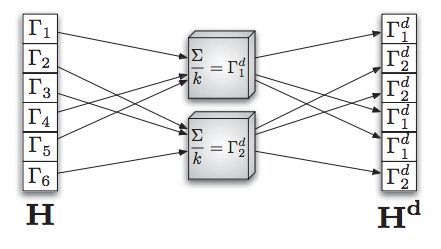
\includegraphics[scale=0.8]{figure/k-same}
		    \caption{Overview of k-same framwork. $H$ is the original image dataset. $H^d$
		    	is the de-identified image dataset.}
		    \label{fig:k-same}
	  	\end{figure}

	  	In $k$-same framework shown as Figure \ref{fig:k-same}, the de-identified result 
	  	of one image in $H^d$ is the average of its $k$ nearest neighbours from a person 
	  	specific image set $H$ \cite{faceDeId09}. In the person-specific image set, each 
	  	person is represented by just one image.

	\subsubsection{K-Same-Pixel$\backslash$Eigen}
	
	E. Newton firstly applied the K-anonymity theory to privacy protectin by de-identifying 
	face images \cite{Newton05}. Claiming that ad-hoc methods, like pixelation, blurring, 
	are not able to protect privacy, they introduced two new approaches based on 
	K-anonymity model: k-Same-Pixel and k-Same-Eigen. These two algorithms are 
	tested in the person specific database that contains only one image for each person. 

	For any one face image, {\it A}, from the person specific database, the process 
	of k-Same-Pixel is:
	\begin{itemize}
		\item Select $k$ face images that are closest to {\it A} including {\it A} itself from the person
				specific database,
		\item Take the average of these $k$ images as ${\it A_{new}}$ by averaging the sum of pixels within
				face regions,
		\item Replace the original image {\it A} with ${\it A_{new}}$,
		\item Repeat the first step if the recognition ratio of A is higher than $\frac{1}{k}$.
	\end{itemize}

	The only difference between k-Same-Pixel and k-Same-Eigen is the later one 
	would take an average image from eigen faces. In mathematics, the eigen face 
	images, composed of eigen values and eigen vectors of original images, are 
	also called projected images, which are computed by Principle Component 
	Analysis (hereinafter referred to as PCA). 

	Compared to ad-hoc approaches, k-Same-Pixel and k-Same-Eigen are able to combat 
	the parrot attack. It is an improvement for privacy protection. However, the
	shortcoming is also very obvious. Due to the different size of multiple faces,
	the de-identified result produced by these two approaches might be a ghost face. 
	Some examples are illustrated in Figure \ref{fig:ghostFace}.
	
	\begin{figure}[!htb]
	    \centering
	    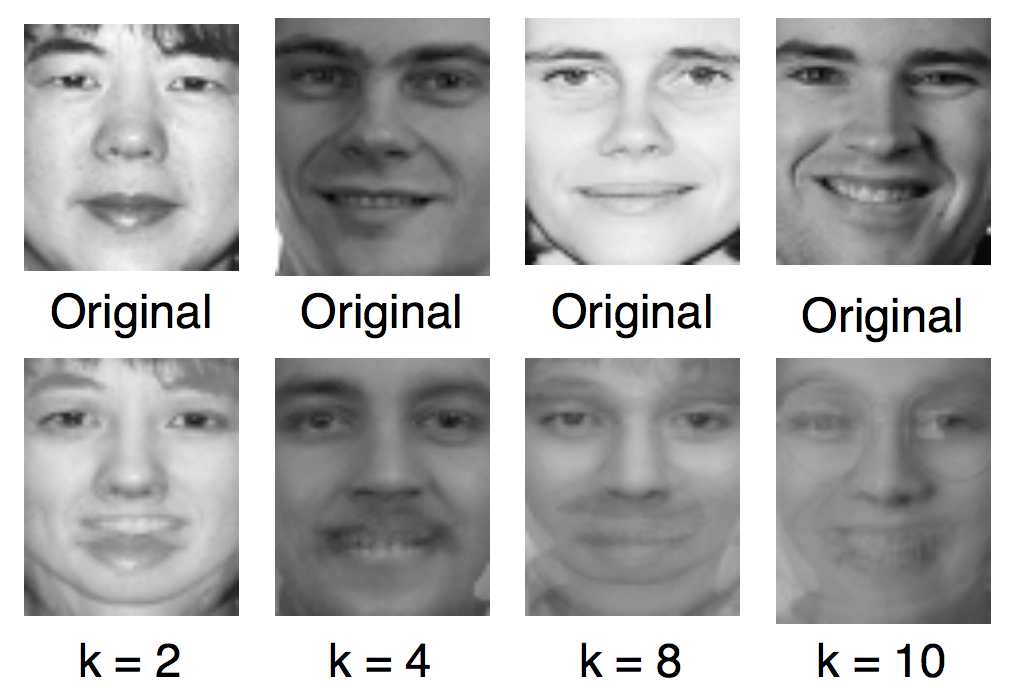
\includegraphics[scale=0.67]{figure/ghostFace}
	    \caption{Ghost face examples. The upper row are the original images. The lower
	    	row are the ghost faces.}
	    \label{fig:ghostFace}
  	\end{figure}

  	Since $k$ faces are stacking together and the face sizes are not the same,
  	the organs in the de-identified face overlaps to form a ghost face. 
  	The de-identified results might be able to combat the automatic face 
  	recognition algorithms for machines. However,
  	the ghost face is totally unreadable and untolerable subjectively. 

	\subsubsection{K-Same-Model}

	K-Same-Model is designed to solve the ghost face problem \cite{Gross08}. 
	This approach combines a model-based face image parameterization with the
	k-same framework. For face images, each one is represented as parameters 
	by the active appearance model, in which the shape and appearance of a 
	face image is represented by parameters separately. The k-same approach 
	is finally applied to these parameters to produce a set of average parameters. 
	At the last step, AAM reconstructs a new face image with the average parameters.
	To describe the procedures clearly, the pseudo code about k-same-model 
	is described as following:
	
	\begin{algorithm}[H]  
	\caption{K-Same-Model Algorithm}  
	\KwIn{A person specific dataset $H$, privacy constant $k$, $|H| \ge k$, 
			Active Appearance Model $\mathcal{A}$}  
	\KwOut{A de-identified dataset $H^d$ }  
	initialization\;
	A new dataset $H_o = \varnothing$ \;
	$H^d = \varnothing$ \;
	\For{$I \in H$}{  
	    Get the AAM parameters representation $c_i$ of $I$ with respect to $\mathcal{A}$\;
	    Add $c_i$ to $H_o$\;
	}  
	\For{$c \in H_o$}
	{
		\If{$|H_o| < 2k$}
		{
			$k = |H_o|$\;
		}

		Select $k$ parameters ${c_1,...,c_k}$ from $H_o$ that are closest 
		to $c$ according to $L_2$ norm\;
		
		$avg = \frac{1}{k}\sum^{k}_{m=1}c_m$\;
		Add $k$ copies of $avg$ to $H_d$\;
		Remove ${c_1,...,c_k}$ from $H_o$\;
	}
	\end{algorithm}

	Since the de-identified processing appears on AAM parameters level, 
	the result is also a set of parameters of a face image. In AAM, shape
	and appearance are constructed as two models. The de-identified
	appearance is finally warped back to de-identified face shape. Therefore,
	the reconstructed face image by AAM is visual natural. 

  	There is an obvious shortcoming in k-Same-Model. This approach might
  	fabricate information that never exists. 

	\begin{figure}[!htb]
	    \centering
	    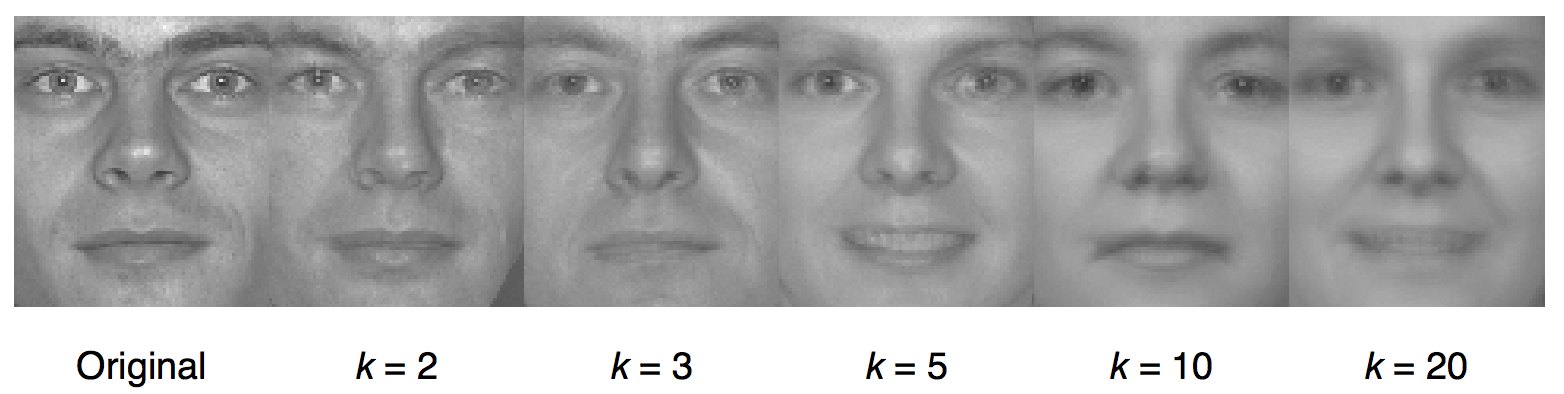
\includegraphics[scale=0.51]{figure/kSameSele}
	    \caption{Shortcomings of k-same-model. Expressions changes when $k=5$
	    	and $k=20$.}
	    \label{fig:kSameSelect}
  	\end{figure}
  	
  	As shown in Figure \ref{fig:kSameSelect}, the original image is a face with
  	neutral expression. When $k=5$, the de-identified result by k-Same-Model is
  	a face with smile expression \cite{faceDeId09}. The reason is that the selected
  	$k$ images have different expressions, so the synthetic face differs from the
  	original one. This example indicates that k-same-model
  	might produce fake information to express different meanings for the original
  	face image.

	\subsubsection{K-Same-Select}

	The previous introduced approaches have shortcomings in preserving data utility,
	such as the ability to recognize the original expressions. 
	In order to solve the trade-off problem between privacy protection and data
	utility preservation in image face de-identification, the k-Same-Select algorithm
	is introduced \cite{Ralph05}. Before taking the average of $k$ images, each face
	is estimated by a utility function. For the images with the same utility scores,
	$k$ images are selected to reconstruct a new face by taking the average. Different
	with k-Same-Model, this approach introduced in \cite{Ralph05} is also 
	appearance-based and works directly on the pixel level. To be more clear, the 
	procedures are described with pseudo code as following:

	\begin{algorithm}[H]  
	\caption{K-Same-Select Algorithm}  
	\KwIn{A person specific dataset $H$, privacy constant $k$, $|H| \ge k$, 
			data utility function $u$}  
	\KwOut{A de-identified dataset $H^d$ }  
		$H^d = \varnothing$\;
		Let $H_1,H_2,...,H_l \subset H$ with $H_i = \{x\in H|u(x)=c_i\}$\;
		$H^{d}_{i} = k-same(H_i,k),i=1,2,...,l$\;
		$H^d = \cap_{i=1}^{l}H^{d}_{i}$\;
	\end{algorithm}

	In the algorithm, the utility function is defined according to
	the data utility types that are required to be preserved. For
	example, the utility function is to classify expressions if the 
	required data utility is expression. The k-same procedures are 
	applied to the images with the same expression. Therefore, the
	de-identified result has the same expression with the original
	image.

	\subsubsection{K-Same-Furthest}

	For all the approaches belonging to k-same framework introduced before, 
	the kernel procedure is to take average of $k$ closest images to replace 
	the original one so that the image could not be re-identified. The 
	experiments show that k-same approaches work well for the person specific
	database in which each person has and only has one image. However, 
	the approaches have a common obvious shortcoming. When one person is
	represented by multiple images, the previous k-same approaches fail to
	protect privacy. The reason is easy to understand. The average of $k$ closest 
	images for one person is still that person. Since the de-identified result of
	the previous k-same approaches is taken from $k$ closest images, the previous 
	k-Same approaches are called k-Same-Closest. Aiming at solving the privacy 
	protection problem in k-Same-Closest, the k-Same-Furthest approach
	\cite{Meng14Face,Sun15} takes the average of $k$ furthest images in $L_2$ norm
	to replace the original one. On the other hand, data utility of the result 
	is also the average of the $k$ furthest images. This approach might
	destory the data utility.

	\subsection{Face Synthesis Approaches}

	The k-same approaches protect privacy by substituting the original face region 
	with an average of $k$ images. There are many other approaches that substitute
	the original face region with a synthetic face. This section would introduce
	some face synthesis approaches used in privacy protection including face swapping 
	\cite{swap08}, face aggregation from donors \cite{Mosa14}, GARP face \cite{GARP14}, 
	face de-identification based on multi-factor model \cite{multifactor08} and 
	attribute preserving de-identification method \cite{Attribute15}. 

	Face swapping is a popular and simple method to de-identify face images. 
	The most intuitive explanation of this idea is to replace one person's face 
	with another one. For a target face $A$ and another face $B$, the landmarks 
	such as eye position, nose position is automatically located. Then, all 
	pixels within a face region $B$ is warped to overlap the target face $A$ 
	based on landmarks positions. The research in ~\cite{swap08} shows the 
	result from face swapping could be photorealistic. However, the de-identified 
	result contains other's privacy information. This approach would give out soneone's
	privacy anyway.

	Considering of the shortcoming of face swapping, S. Mosaddegh etc. ~\cite{Mosa14}
	proposes the method that substitutes the original face with a synthetic face 
	composing of several donors' face parts, such as eyes, nose, mouth. Since the 
	synthetic face contains several persons' characters, it succeeds to deceive 
	machine recognition algorithms and humans without leaking anyone's privacy.
	Nevertheless, this approach does not consider the problem of data utility 
	preservation.

	To balance the privacy protection and data utility preservation, a multi-factor 
	model is used to separate privacy related factors and non-privacy related ones 
	\cite{multifactor08}. During the de-identification processing, only the privacy related 
	factors are altered with the non-privacy factors untouched. The multi-factor 
	model in \cite{multifactor08} is the combination of linear model, bilinear model 
	and quadratic model. Theoretically, the multi-factor model works when only two data 
	utilities appear in the database. This approach can not guarantee the ability when 
	more types of images are included.

	For the image dataset with multiple data utilities, the specific details are
	processed individually. In \cite{GARP14}, gender (G), age (A), race (R) are
	classified and only the images with the same GAR are blended as the de-identified
	result. In \cite{Attribute15}, images are classified according to 17 attributes 
	including gender, race, hair color etc firstly. Then the images with the similar
	attributes are de-identified. In a summary, the GARP face and attribute preserving
	algorithm are both similar to k-Same-Select approach.      

\section{Approaches for Videos}
\label{sec:APPvideos}

	Traditional approaches of protecting privacy in videos are to blur or mask the face regions manually which is very 
	cumbersome and time consuming..
	Since large amount of video data are producing quickly, automatic face de-identifying method for videos becomes very important.
	The existing methods follow the same basic structure. That is to detect face regions in
	all frames and then apply the image obfuscation algorithm. Because of the simplicity, these methods 
  	are widely used in practical situations such as TV interviews or surveillance videos \cite{Agrawal09}. Except
  	for pixelation and blurring, encryption and video scrambling are also general methods to obfuscate
  	face regions\cite{TrustCam10,dufaux10,scram11}. Figure \ref{fig:encrypt} shows a encrypted frame from a video.

	\begin{figure}[!htb]
	    \centering
	    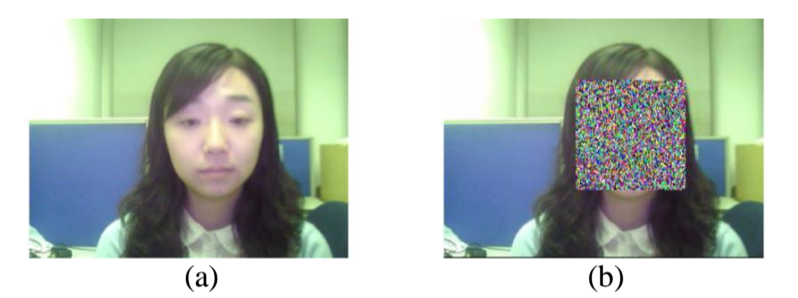
\includegraphics{figure/encrypt}
	    \caption{One encryption frame. (a) is the original image. (b) is the 
	    	encrypted image in which face region is covered by snow board.}
	    \label{fig:encrypt}
  	\end{figure}

  	Inferred from above analysis, only the ad-hoc methods for images are applied to videos. The other algorithms
	of face de-identification in images are not suitable to process videos, because after de-identification the identity 
	cannot be kept invariant for adjacent images. It would be strange if a person's face changes all the time
	when a video is playing.
	